% cuRAMSES: Scalable Domain Decomposition and Memory-Efficient AMR
% for Cosmological Simulations
%
% MNRAS-style LaTeX paper
%
\documentclass[fleqn,usenatbib]{mnras}

% Standard packages
\usepackage{amsmath,amssymb}
\usepackage{graphicx}
\usepackage{algorithm}
\usepackage{algorithmic}
\usepackage{booktabs}
\usepackage{multirow}
\usepackage{xcolor}
\usepackage{hyperref}

% Algorithm formatting
\renewcommand{\algorithmicrequire}{\textbf{Input:}}
\renewcommand{\algorithmicensure}{\textbf{Output:}}

% Shorthand macros
\newcommand{\ramses}{\textsc{ramses}}
\newcommand{\curamses}{\textsc{cuRAMSES}}
\newcommand{\ncpu}{N_{\rm cpu}}
\newcommand{\ngridmax}{N_{\rm gridmax}}
\newcommand{\nlevelmax}{N_{\rm levelmax}}
\newcommand{\twotondim}{2^{N_{\rm dim}}}
\newcommand{\ksec}{k\text{-section}}
\newcommand{\Olog}[1]{\mathcal{O}(#1)}
\newcommand{\code}[1]{\texttt{#1}}

\title[cuRAMSES: Scalable AMR for Cosmological Simulations]
{cuRAMSES: Scalable Domain Decomposition and Memory-Efficient AMR
for Cosmological Simulations}

\author[J.~Kim]{
Juhan Kim$^{1}$\thanks{E-mail: kjhan@kias.re.kr}
\\
$^{1}$Center for Advanced Computation, Korea Institute for Advanced Study,
85 Hoegiro, Dongdaemun-gu, Seoul 02455, Republic of Korea
}

\date{Accepted XXX. Received YYY; in original form ZZZ}

\pubyear{2026}

\begin{document}

\label{firstpage}
\pagerange{\pageref{firstpage}--\pageref{lastpage}}

\maketitle

% ===================================================================
% ABSTRACT
% ===================================================================
\begin{abstract}
We present \curamses, a suite of algorithmic and implementation
improvements to the \ramses\ adaptive mesh refinement (AMR)
cosmological simulation code that address the principal bottlenecks
encountered in large-scale simulations: communication overhead, memory
consumption, and solver efficiency. The central innovation is a
recursive \ksec\ domain decomposition that replaces the traditional
Hilbert curve ordering with a hierarchical spatial partitioning,
dramatically reducing the number of MPI messages per ghost-zone
exchange and eliminating all \code{MPI\_ALLTOALL} calls. A Morton key
hash table for octree neighbour lookup removes one of the largest
per-rank arrays in the original code, while on-demand allocation
strategies for auxiliary arrays further reduce the memory footprint.
Optimizations to the multigrid Poisson solver --- including precomputed
neighbour caches, merged communication steps, and fused computation
kernels --- substantially lower its share of total runtime. A spatial
hash binning scheme accelerates Type~II supernova and AGN feedback by
orders of magnitude over the original brute-force approach. We also
implement variable-$\ncpu$ restart via HDF5 parallel I/O, removing the
constraint that checkpoint files must be read with the same number of
MPI ranks as were used to write them. All modifications preserve
physical consistency, as verified by conservation-law diagnostics
across extensive test suites.
\end{abstract}

\begin{keywords}
methods: numerical -- cosmology: simulations -- hydrodynamics --
software: development
\end{keywords}

% ===================================================================
% 1. INTRODUCTION
% ===================================================================
\section{Introduction}
\label{sec:intro}

Cosmological hydrodynamic simulations play a central role in modern
astrophysics, connecting the predictions of the $\Lambda$CDM paradigm
to the observable properties of galaxies, the intergalactic medium,
and the large-scale structure of the Universe
\citep{Vogelsberger2014,Schaye2015,Dubois2014}. Adaptive mesh
refinement (AMR) codes such as \ramses\ \citep{Teyssier2002} provide
an attractive framework for these simulations: the computational mesh
is refined only where the physics demands it, concentrating resources
on collapsing haloes and star-forming regions while keeping the cost
of smooth, low-density regions manageable.

However, scaling AMR codes to the regime of $10^{10}$--$10^{11}$
particles and $10^4$--$10^5$ MPI ranks poses several intertwined
challenges:

\begin{enumerate}
\item \emph{Communication scaling.} The standard \ramses\
  domain decomposition is based on a Hilbert space-filling curve.
  Ghost-zone (virtual boundary) exchange requires every rank to
  communicate its emission and reception lists to \emph{all} other
  ranks via \code{MPI\_ALLTOALL}, leading to
  $\Olog{\ncpu^2}$ message complexity and a corresponding memory
  footprint of $\Olog{\ncpu}$ per-rank buffers.

\item \emph{Memory overhead.} Several large arrays in \ramses\
  scale linearly with $\ngridmax$, the maximum number of AMR grids per
  rank. The neighbour-pointer array \code{nbor($\ngridmax$, 6)}
  alone consumes $48\,\ngridmax$ bytes; the Hilbert key array adds
  another $16\,\ngridmax$ bytes when compiled with
  \code{QUADHILBERT}. For production runs with
  $\ngridmax \sim 5 \times 10^6$, these arrays together consume
  nearly 1\,GB per rank --- memory that could otherwise accommodate
  more particles or finer refinement.

\item \emph{Load balancing flexibility.} The Hilbert ordering
  distributes computational load based on cell count alone. In
  practice, the memory consumed by a grid cell depends on both the
  grid data structures (hydro variables, gravity arrays, linked lists)
  and the number of particles attached to the cell. A cell hosting
  $10^4$ particles in a dense halo is far more expensive in memory
  than a void cell with zero particles, yet the standard load balancer
  treats them equally.

\item \emph{Solver efficiency.} The multigrid Poisson solver
  typically dominates runtime in gravity-coupled simulations. Its
  per-iteration cost is driven not only by floating-point operations
  but also by frequent ghost-zone exchanges (up to nine per smoothing
  iteration) and repeated hash table lookups for neighbour grids in the
  octree.

\item \emph{Checkpoint flexibility.} \ramses\ writes one file per
  MPI rank. Restarting with a different number of ranks requires an
  intermediate dump-and-redistribute step, which is cumbersome for
  production workflows where available node counts vary between
  allocations.
\end{enumerate}

In this paper we describe \curamses, a comprehensive set of
modifications to \ramses\ that addresses each of these challenges. The
key innovations are:

\begin{itemize}
\item A recursive \ksec\ domain decomposition (Section~\ref{sec:ksection}) that
  replaces Hilbert ordering with a hierarchical multi-way spatial
  partitioning, enabling hierarchical MPI exchange with
  $\Olog{\sum_l k_l}$ messages per operation.

\item A Morton key hash table for octree neighbour lookup
  (Section~\ref{sec:morton}) that eliminates the \code{nbor} array
  entirely, saving $\sim$240\,MB per rank at $\ngridmax = 5 \times
  10^6$.

\item On-demand allocation and elimination of redundant large arrays
  (Section~\ref{sec:memory}), yielding over 1\,GB of additional
  savings per rank.

\item Algorithmic optimizations to the multigrid Poisson solver
  (Section~\ref{sec:multigrid}), reducing its share of total runtime
  from 55\,per\,cent to 39\,per\,cent.

\item A spatial hash binning scheme for Type~II supernova and AGN
  feedback (Section~\ref{sec:feedback}), accelerating the feedback
  averaging and blast injection by orders of magnitude.

\item Variable-$\ncpu$ restart with HDF5 parallel I/O
  (Section~\ref{sec:varcpu}), along with miscellaneous improvements
  described in Section~\ref{sec:misc}.
\end{itemize}

Performance benchmarks are presented in
Section~\ref{sec:performance}, and we conclude in
Section~\ref{sec:conclusions}.

Throughout this paper, we use the notation of \citet{Teyssier2002}:
$\nlevelmax$ is the maximum AMR level, $\ngridmax$ is the maximum
number of grids per rank, \code{twotondim} $= 2^{N_{\rm dim}} = 8$
is the number of cells per oct in three dimensions, and
$\ncpu$ is the total number of MPI ranks.


% ===================================================================
% 2. K-SECTION DOMAIN DECOMPOSITION
% ===================================================================
\section{Recursive K-Section Domain Decomposition}
\label{sec:ksection}

\subsection{Motivation}
\label{sec:ksec_motivation}

The standard \ramses\ domain decomposition assigns cells to MPI ranks
by sorting them along a Hilbert space-filling curve and partitioning
the resulting one-dimensional index range into $\ncpu$ contiguous
segments. While this preserves spatial locality reasonably well, it
has two significant drawbacks for large-scale runs:

\begin{enumerate}
\item The ghost-zone exchange requires \code{MPI\_ALLTOALL} to
  communicate emission/reception counts, followed by point-to-point
  messages to all ranks with non-zero counts. In the worst case, every
  rank communicates with every other rank, yielding $\Olog{\ncpu^2}$
  total messages.

\item The Hilbert key computation requires a large per-rank array
  \code{hilbert\_key(1:ncell)} of 16 bytes per cell (when compiled
  with \code{QUADHILBERT}), totalling $\sim$640\,MB at
  $\ngridmax = 5 \times 10^6$.
\end{enumerate}

Our recursive \ksec\ decomposition replaces the one-dimensional Hilbert
partitioning with a recursive spatial partitioning in the original
three-dimensional coordinate space. This produces a $k$-ary tree whose
structure directly encodes the communication pattern, enabling
hierarchical message routing that scales with the tree depth rather
than the total number of ranks.


\subsection{Tree construction}
\label{sec:ksec_tree}

Given $\ncpu$ MPI ranks, we first compute the prime factorization:
\begin{equation}
\ncpu = p_1^{m_1} \times p_2^{m_2} \times \cdots \times p_r^{m_r},
\quad p_1 > p_2 > \cdots > p_r.
\label{eq:prime_factorization}
\end{equation}
The splitting sequence is then
\begin{equation}
\mathbf{k} = (\underbrace{p_1, \ldots, p_1}_{m_1},
              \underbrace{p_2, \ldots, p_2}_{m_2}, \ldots,
              \underbrace{p_r, \ldots, p_r}_{m_r}),
\label{eq:split_sequence}
\end{equation}
yielding $L = \sum_i m_i$ levels in the tree. At each level $l$, the
domain is split into $k_l$ sub-domains along the longest axis of the
current bounding box. This longest-axis selection ensures roughly
isotropic sub-domains, minimizing the surface-to-volume ratio and
hence the ghost-zone count.

For example, $\ncpu = 12 = 3 \times 2 \times 2$ produces the
splitting sequence $(3, 2, 2)$ with $L = 3$ tree levels: the root is
split into 3 slabs along the longest axis, each slab is bisected, and
each half is bisected again, yielding 12 leaf nodes --- one per rank.
Fig.~\ref{fig:ksec_progressive} illustrates this progressive
decomposition for $\ncpu = 12$, from the undivided domain through
three successive levels of splitting, with the corresponding
\ksec\ tree shown beneath each panel.

\begin{figure}
\centering
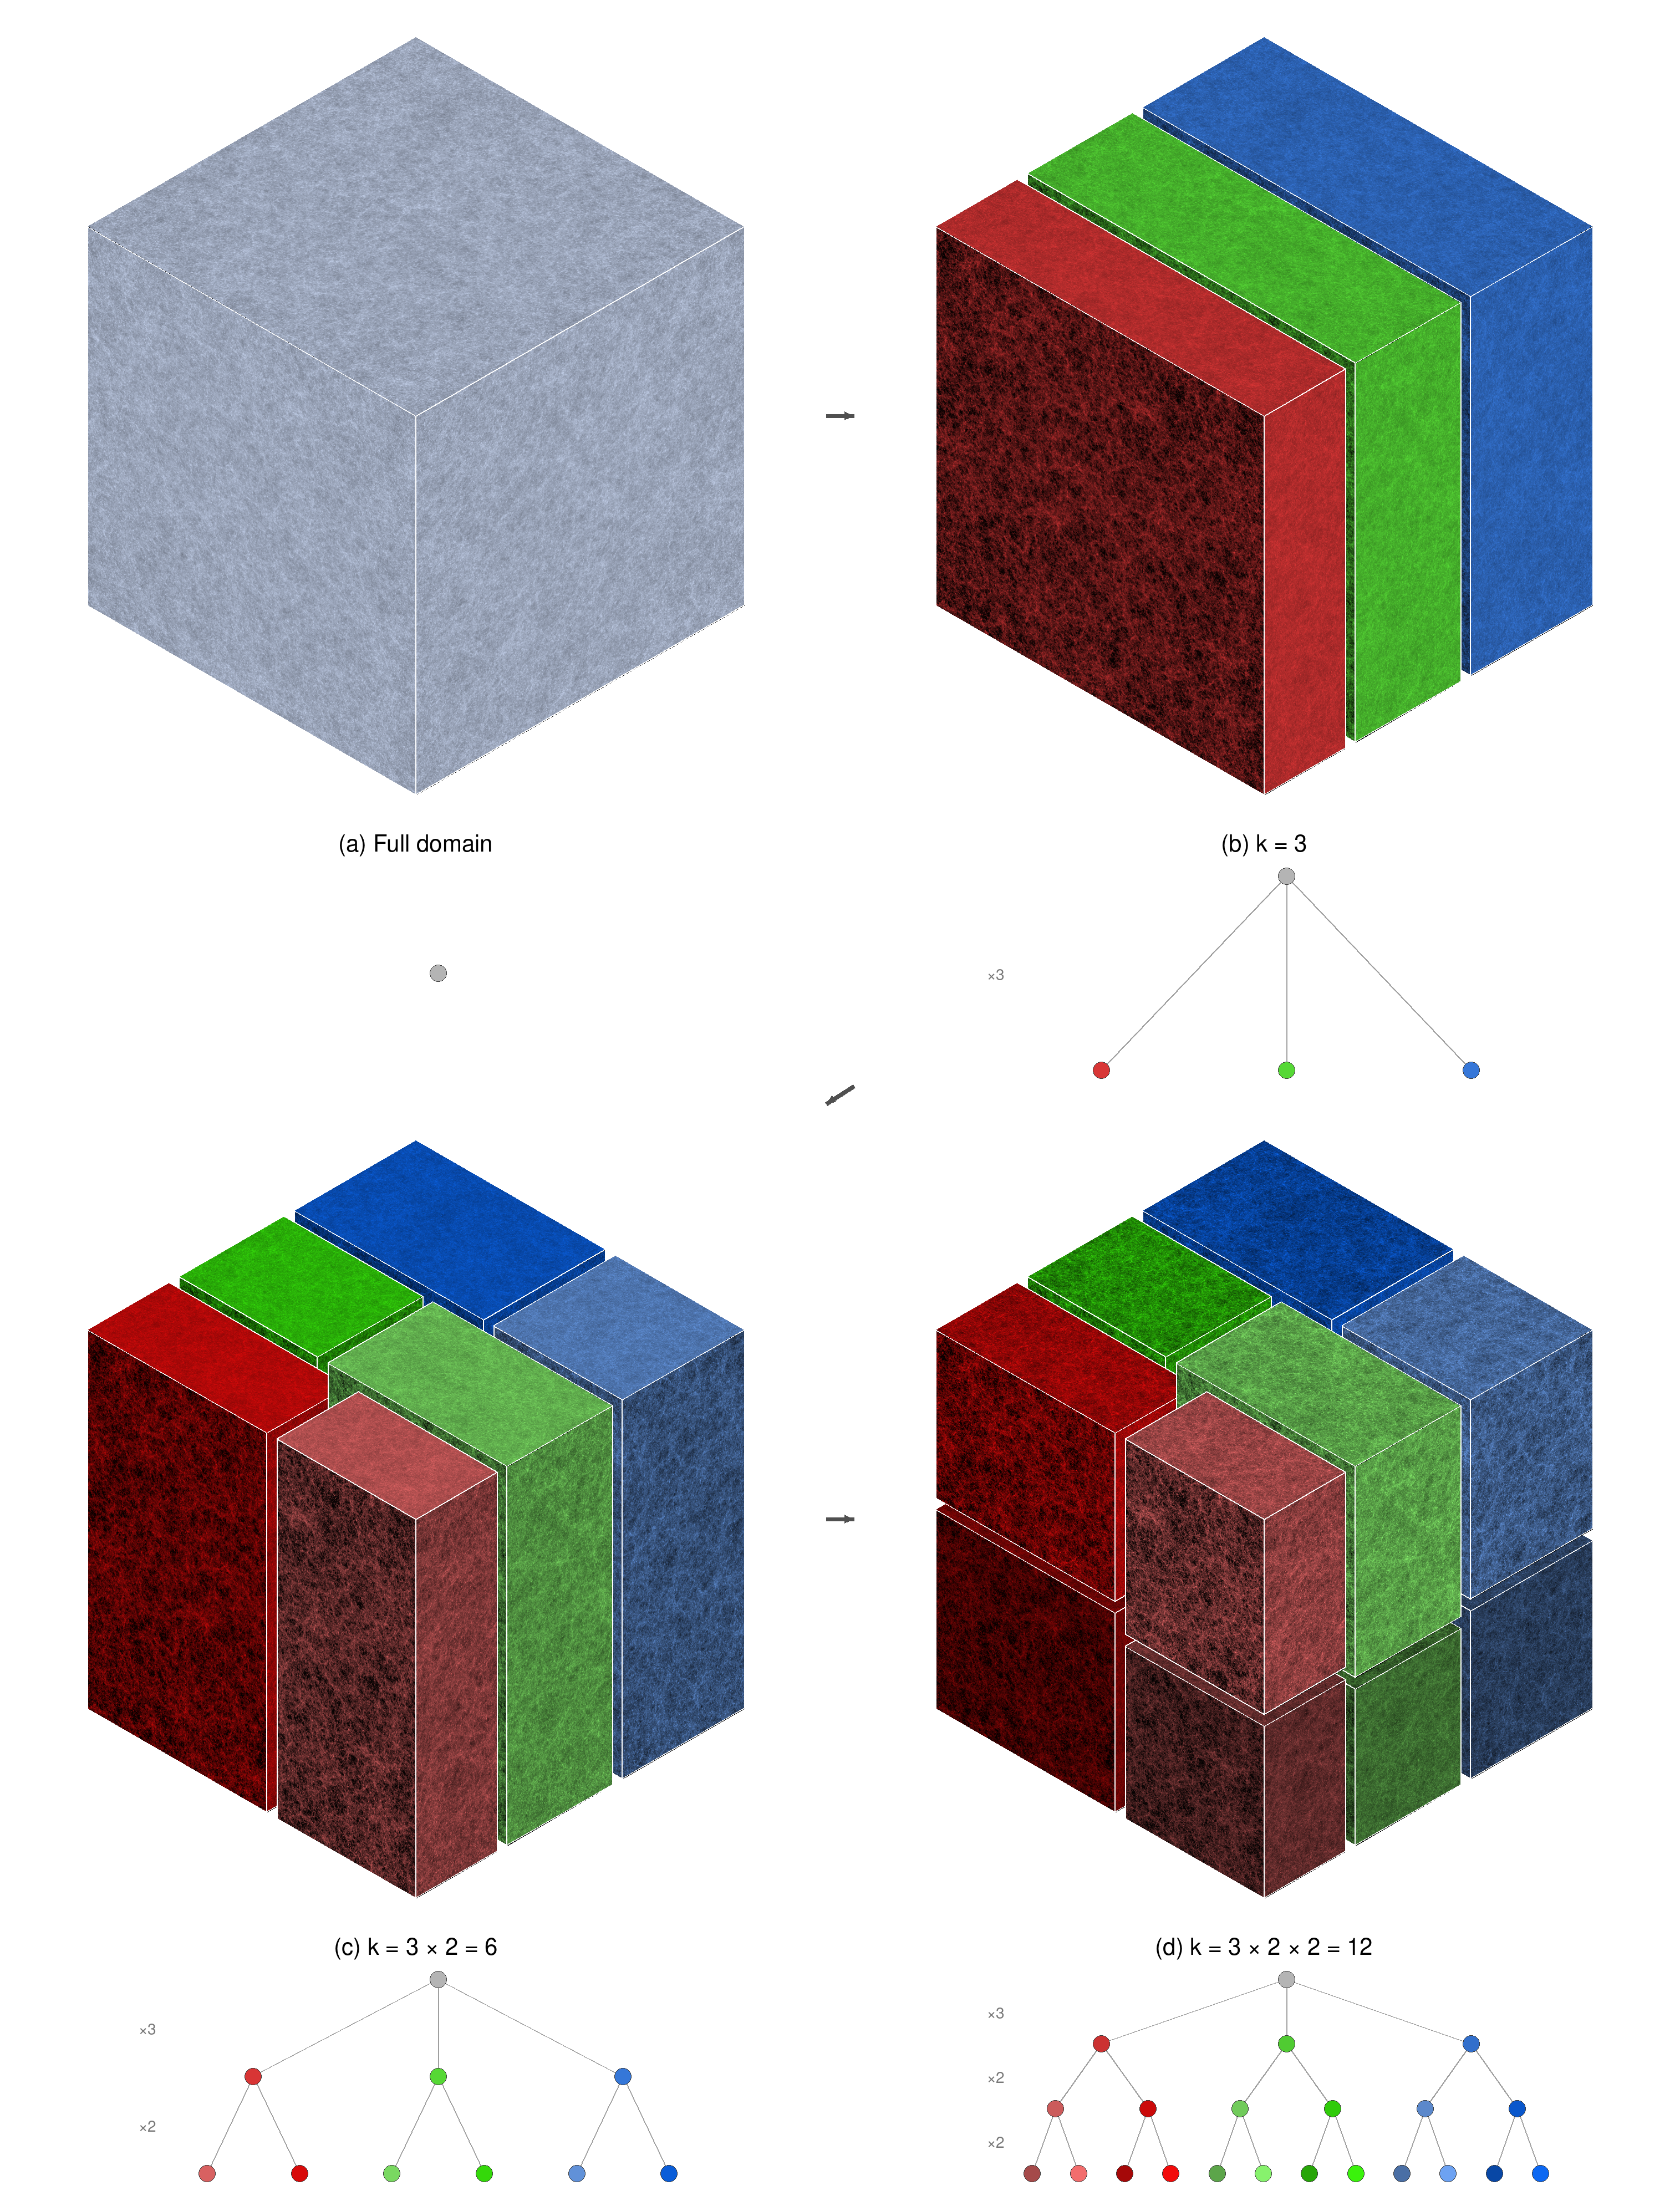
\includegraphics[width=\columnwidth]{../misc/ksection_progressive.png}
\caption{Progressive recursive \ksec\ decomposition for $\ncpu = 12 =
3 \times 2 \times 2$. (a)~The undivided simulation domain. (b)~First
split into $k = 3$ slabs along the longest axis. (c)~Each slab bisected
along the second axis ($3 \times 2 = 6$ sub-domains). (d)~Final bisection
along the third axis ($3 \times 2 \times 2 = 12$ leaf domains). Below
each panel, the corresponding \ksec\ tree is shown; colours encode
$x$-slab membership (red/green/blue), with saturation and brightness
indicating $y$ and $z$ subdivisions. Each face displays projected
column density from a $4096^3$ TSC density field. Sub-domain volumes
vary by ${\sim}10$--$30\,\%$, reflecting load-balanced wall placement.}
\label{fig:ksec_progressive}
\end{figure}

The tree is stored as a set of arrays indexed by node identifier:
\begin{itemize}
\item \code{ksec\_next(node, j)}: child node index for partition $j$
  ($j = 1, \ldots, k_l$);
\item \code{ksec\_wall(node, j)}: spatial coordinate of the $j$-th
  partition boundary within the node's extent;
\item \code{ksec\_indx(leaf)}: the MPI rank assigned to a leaf node;
\item \code{ksec\_cpumin(node)}, \code{ksec\_cpumax(node)}: range of
  MPI ranks contained in the subtree rooted at this node.
\end{itemize}

The total number of tree nodes is
\begin{equation}
N_{\rm nodes} = 1 + \sum_{l=1}^{L} \prod_{i=1}^{l} k_i \leq
1 + L \cdot k_{\rm max}^L,
\label{eq:tree_nodes}
\end{equation}
which for practical values ($\ncpu \leq 10^5$) is at most a few
hundred --- negligible overhead.


\subsection{Load-balanced wall placement}
\label{sec:ksec_loadbal}

When the tree is updated during load balancing (every \code{nremap}
coarse steps), the wall positions are adjusted by iterative
dichotomy so that each partition receives a load proportional to the
number of ranks it contains.

The procedure operates level by level, top to bottom. At level $l$:

\begin{enumerate}
\item A histogram is built over the splitting coordinate: for each
  node at level $l$, the cells within that node are projected onto the
  splitting axis and binned into a cumulative cost histogram with
  resolution $\Delta x_{\rm hist}$.

\item For each of the $k_l - 1$ walls within each node, a binary
  search (dichotomy) adjusts the wall position until the cumulative
  load on the left side matches the target fraction. The target
  cumulative fraction for wall $j$ in a node spanning ranks
  $[i_{\rm min}, i_{\rm max}]$ with total count
  $n = i_{\rm max} - i_{\rm min} + 1$ is
  \begin{equation}
  f_j = \frac{\sum_{m=1}^{j} n_m}{n},
  \label{eq:target_frac}
  \end{equation}
  where $n_m$ is the number of ranks assigned to partition $m$
  ($n_m = \lfloor n/k_l \rfloor$ or $\lfloor n/k_l \rfloor + 1$ for
  the first $n \bmod k_l$ partitions).

\item An \code{MPI\_ALLREDUCE} aggregates the local histograms across
  all ranks to obtain the global cumulative load at each wall
  position. The dichotomy converges when the relative load imbalance
  $|\hat{L}_j - L_j^{\rm target}| / L_j^{\rm target}$ falls below a
  tolerance $\epsilon_{\rm tol}$ (typically $10^{-2}$), or when the
  wall position can no longer be resolved at the histogram resolution.

\item After wall convergence, the cells are repartitioned (sorted)
  according to the new wall positions, and the histogram bounds are
  updated for the next level.
\end{enumerate}


\subsection{Memory-weighted cost function}
\label{sec:ksec_membal}

The default \ramses\ load balancer weights all cells equally.
\curamses\ supports an optional memory-weighted cost function:
\begin{equation}
C_{\rm cell} = \frac{w_{\rm grid}}{\twotondim} +
\frac{n_{\rm part}({\rm igrid}) \cdot w_{\rm part}}{\twotondim},
\label{eq:cost_function}
\end{equation}
where $w_{\rm grid}$ is the memory cost per grid slot (default 270
bytes, accounting for hydro, gravity, and AMR bookkeeping arrays),
$w_{\rm part}$ is the memory cost per particle slot (default 12 bytes
for position, velocity, mass, and linked-list pointers), and
$n_{\rm part}({\rm igrid})$ is the number of particles attached to
grid \code{igrid}. The division by $\twotondim$ distributes the grid
cost evenly among its eight cells.

This cost function ensures that ranks hosting dense haloes (many
particles per cell) receive fewer cells, preventing memory exhaustion
on particle-heavy ranks. All histogram loads are accumulated in 64-bit
integers to avoid overflow when summing costs across millions of cells.

Activating memory-weighted balancing requires setting
\code{memory\_balance = .true.} and optionally tuning
\code{mem\_weight\_grid} and \code{mem\_weight\_part} in the namelist.
Our tests with $2 \times 10^8$ particles on 12 ranks show that
memory-weighted balancing reduces the peak-to-mean memory ratio from
2.5 to 1.3 without affecting physics results (identical
$e_{\rm cons}$, $e_{\rm pot}$, $e_{\rm kin}$ to machine precision).


\subsection{Hierarchical MPI exchange}
\label{sec:ksec_exchange}

The tree structure enables a hierarchical exchange protocol that
replaces the global \code{MPI\_ALLTOALL} with a sequence of
level-by-level correspondent exchanges. We implement two variants:

\subsubsection{Exclusive exchange}
\label{sec:ksec_exclusive}

In the exclusive exchange (\code{ksection\_exchange\_dp}), each item
has a unique destination rank. The algorithm walks the tree from root
to leaf:

\begin{algorithm}[H]
\caption{Exclusive hierarchical exchange}
\label{alg:exclusive}
\begin{algorithmic}[1]
\REQUIRE Send buffer $\mathbf{S}$ with $N$ items, destination ranks $\mathbf{d}$
\ENSURE Receive buffer $\mathbf{R}$ with items destined for this rank
\STATE $\mathbf{W} \leftarrow \mathbf{S}$; $\mathbf{D} \leftarrow \mathbf{d}$; node $\leftarrow$ root
\FOR{$l = 1$ \TO $L$}
  \STATE $k \leftarrow k_l$; my\_child $\leftarrow$ \code{ksec\_cpu\_path}(myid, $l$)
  \STATE Classify items in $\mathbf{W}$ by child index (counting sort on $\mathbf{D}$)
  \STATE Identify $k-1$ correspondent ranks (one per sibling child)
  \FOR{each correspondent $p$}
    \STATE Exchange count: \code{MPI\_ISEND/IRECV} (tag $100+l$)
    \STATE Exchange data: \code{MPI\_ISEND/IRECV} (tags $200+l$, $300+l$)
  \ENDFOR
  \STATE \code{MPI\_WAITALL}
  \STATE $\mathbf{W} \leftarrow$ merge(my\_child items, received items)
  \STATE node $\leftarrow$ \code{ksec\_next}(node, my\_child)
\ENDFOR
\STATE $\mathbf{R} \leftarrow \mathbf{W}$
\end{algorithmic}
\end{algorithm}

At each level, each rank communicates with at most $k_l - 1$
correspondent ranks (one from each sibling subtree). The
correspondent in a sibling subtree of size $s$ is chosen as
$\min(\text{my\_pos}, s-1)$ to distribute load evenly. The total
number of messages per rank per exchange is
\begin{equation}
N_{\rm msg} = \sum_{l=1}^{L} (k_l - 1) = \sum_i m_i (p_i - 1),
\label{eq:msg_count}
\end{equation}
which for $\ncpu = 1024 = 2^{10}$ gives $N_{\rm msg} = 10$, compared
to $\Olog{1024}$ messages in the original all-to-all pattern.

Working buffers are managed with Fortran 2003 \code{move\_alloc} for
zero-copy buffer swaps at each level, and per-level arrays (child
counts, peer lists, MPI request handles) are pre-allocated with
\code{save} attributes to eliminate allocation/deallocation overhead
on repeated calls.


\subsubsection{Overlap exchange}
\label{sec:ksec_overlap}

The overlap exchange (\code{ksection\_exchange\_dp\_overlap}) handles
items with spatial extent (bounding boxes) that may overlap multiple
sub-domains. At each tree level, an item is replicated to all children
whose bounding box intersects the item's spatial extent. This is used
for operations such as the supernova feedback, where each SN blast
has a finite physical radius.

To handle periodic boundary conditions, items near the domain boundary
are pre-processed: for each wrapping dimension, shifted copies are
generated using bitmask subset enumeration over the set of wrapping
dimensions:
\begin{equation}
N_{\rm copies} = 2^{n_{\rm wrap}} - 1,
\label{eq:periodic_copies}
\end{equation}
where $n_{\rm wrap}$ is the number of dimensions in which the item's
extent crosses the periodic boundary. This ensures correct routing
without modifying the tree walk itself.


\subsection{Ghost-zone exchange via k-section}
\label{sec:ksec_ghostzone}

The ghost-zone (virtual boundary) exchange is the most
communication-intensive operation in \ramses, called multiple times per
fine time step for hydro, gravity, and particle updates. We replace
the standard all-to-all pattern with four \ksec-based routines:

\begin{itemize}
\item \code{make\_virtual\_fine\_dp\_ksec}: forward exchange (emission
  grids $\rightarrow$ reception grids).
\item \code{make\_virtual\_reverse\_dp\_ksec}: reverse accumulation
  (reception grids $\rightarrow$ emission grids, with \code{+=}
  semantics).
\item \code{make\_virtual\_fine\_int\_ksec}: integer variant (via
  \code{int} $\rightarrow$ \code{dble} conversion, exchange, then
  \code{nint} inverse).
\item Multigrid variants: \code{make\_virtual\_mg\_dp\_ksec} and
  \code{make\_reverse\_mg\_dp\_ksec} for the multigrid solver's active
  and emission grid structures.
\end{itemize}

The data packing format for each ghost grid is:
\begin{equation}
\text{sendbuf}(1:\twotondim+2,\, i) = \bigl\{
u_1, \ldots, u_{\twotondim},\, \text{sender\_id},\, \text{index}
\bigr\},
\label{eq:sendbuf_format}
\end{equation}
where $u_j$ are the cell data values, \code{sender\_id} identifies the
source rank, and \code{index} is the emission or reception array index
used for scatter at the receiver. This self-describing format enables
the receiver to place incoming data without maintaining separate
communication tables.


\subsection{Bulk exchange}
\label{sec:ksec_bulk}

For multi-variable exchanges (e.g., all hydro conserved variables), we
provide bulk variants that pack all $N_{\rm var}$ columns of a 2D
array into a single \ksec\ exchange call:
\begin{equation}
\text{sendbuf}\bigl((v-1)\twotondim + j,\, i\bigr) =
\text{xx}(v,\, \text{cell}_{i,j}),
\label{eq:bulk_format}
\end{equation}
for $v = 1, \ldots, N_{\rm var}$ and $j = 1, \ldots, \twotondim$,
plus two metadata entries. This amortizes the tree-walk overhead and
MPI latency over $N_{\rm var}$ variables, yielding a significant
reduction in the number of exchange calls per time step (from
$N_{\rm var}$ individual calls to a single bulk call at each of the
five call sites in \code{amr\_step}).

For MHD simulations (\code{SOLVERmhd}), the bulk exchange handles
$N_{\rm var} + 3$ columns to include the face-centred magnetic field
components.


\subsection{Communication structure construction}
\label{sec:ksec_buildcomm}

The construction of the communication structure (\code{build\_comm})
--- which determines which grids must be exchanged as ghost zones ---
was itself based on \code{MPI\_ALLTOALL} in the original \ramses. We
replace this with a \ksec\ exchange: each rank packs its reception
grids as triplets (sender\_id, reception\_index, grid\_address), sends
them via \code{ksection\_exchange\_dp}, and the receiver reconstructs
its emission arrays from the incoming data. This eliminates the last
remaining all-to-all communication pattern in the AMR infrastructure.


\subsection{Complexity analysis}
\label{sec:ksec_complexity}

Table~\ref{tab:complexity} summarizes the communication complexity of
the original \ramses\ and \curamses.

\begin{table}
\centering
\caption{Communication complexity per ghost-zone exchange operation.
$N_{\rm ghost}$ is the total number of ghost grids per rank; $k_l$
are the branching factors at tree level $l$.}
\label{tab:complexity}
\begin{tabular}{lcc}
\toprule
& Original \ramses & \curamses \\
\midrule
Message count & $\Olog{\ncpu}$ & $\Olog{\sum_l k_l}$ \\
Buffer memory & $\Olog{\ncpu \cdot N_{\rm ghost}}$ &
  $\Olog{k_{\rm max} \cdot N_{\rm ghost}}$ \\
\code{MPI\_ALLTOALL} calls & $\geq 1$ per exchange & 0 \\
\bottomrule
\end{tabular}
\end{table}


% ===================================================================
% 3. MORTON KEY OCTREE
% ===================================================================
\section{Morton Key Octree for Neighbour Lookup}
\label{sec:morton}

\subsection{The nbor array problem}
\label{sec:morton_problem}

\ramses\ stores the octree connectivity in several arrays, the largest
of which is \code{nbor(1:ngridmax, 1:twondim)} --- a six-column
integer array that records, for each grid, the cell index of its
neighbour in each of the six Cartesian directions ($\pm x$, $\pm y$,
$\pm z$). At 8 bytes per entry (64-bit integers), this array consumes
\begin{equation}
M_{\rm nbor} = 6 \times 8 \times \ngridmax = 48\,\ngridmax
\text{ bytes.}
\label{eq:nbor_memory}
\end{equation}
For $\ngridmax = 5 \times 10^6$, this is 240\,MB per rank. Moreover,
the \code{nbor} array must be maintained during grid creation,
deletion, defragmentation, and inter-rank migration --- a significant
source of code complexity and a potential source of bugs.


\subsection{Morton key encoding}
\label{sec:morton_encoding}

A Morton key (also known as a Z-order key) is a 64-bit integer formed
by interleaving the bits of the three-dimensional integer coordinates
$(i_x, i_y, i_z)$ of a grid at its AMR level:
\begin{equation}
M(i_x, i_y, i_z) = \sum_{b=0}^{B-1}
\Bigl[
  \text{bit}_b(i_x) \cdot 2^{3b} +
  \text{bit}_b(i_y) \cdot 2^{3b+1} +
  \text{bit}_b(i_z) \cdot 2^{3b+2}
\Bigr],
\label{eq:morton_encode}
\end{equation}
where $B = 21$ bits per coordinate (supporting grids up to level 22
for $n_x = 1$, or level 20 for $n_x = 4$), and $\text{bit}_b(n)$
extracts bit $b$ of integer $n$. The encoding and decoding are
implemented with simple bit-shift loops.

The integer coordinates of a grid at level $l$ are computed from its
floating-point centre position $\mathbf{x}_g$ as
\begin{equation}
i_d = \lfloor x_{g,d} \cdot 2^{l-1} \rfloor, \quad d \in \{x, y, z\},
\label{eq:grid_to_int}
\end{equation}
where coordinates are in units of the coarse grid spacing.


\subsection{Neighbour finding via Morton arithmetic}
\label{sec:morton_neighbor}

The neighbour of a grid in direction $j$ (using the \ramses\ convention
$1 = -x$, $2 = +x$, $3 = -y$, $4 = +y$, $5 = -z$, $6 = +z$) is
obtained by:
\begin{enumerate}
\item Decoding the Morton key to $(i_x, i_y, i_z)$.
\item Incrementing or decrementing the appropriate coordinate.
\item Applying periodic wrapping if the coordinate exceeds
  $[0, n_d \cdot 2^{l-1})$.
\item Re-encoding to obtain the neighbour's Morton key.
\end{enumerate}

The parent key is obtained by a 3-bit right shift: $M_{\rm parent} =
M \gg 3$. A child key is obtained by a 3-bit left shift plus the
child index (0--7): $M_{\rm child} = (M \ll 3) \,|\, i_{\rm child}$.


\subsection{Per-level hash table}
\label{sec:morton_hashtable}

We maintain one open-addressing hash table per AMR level, mapping
Morton keys to grid indices:
\begin{equation}
\text{mort\_table}(l) : M \mapsto \text{igrid}.
\label{eq:hash_table}
\end{equation}

The hash function uses multiplicative hashing with Knuth's golden
ratio constant and an additional mixing step:
\begin{equation}
h(M) = \bigl[\bigl((M \times \phi_1) \oplus (M \gg 16)\bigr) \times
\phi_2\bigr] \oplus (h \gg 13),
\label{eq:hash_func}
\end{equation}
where $\phi_1 = 2654435761$ and $\phi_2 = \texttt{0x9E3779B97F4A7C15}$
are constants chosen for good bit mixing, and the table capacity is
always a power of two to allow bitmask modular arithmetic. Collisions
are resolved by linear probing; the load factor is kept below 0.7 by
automatic rehashing (doubling capacity).

The hash table is maintained incrementally:
\begin{itemize}
\item \code{morton\_hash\_insert}: called during \code{make\_grid\_coarse} and \code{make\_grid\_fine};
\item \code{morton\_hash\_delete}: called during \code{kill\_grid};
\item Full rebuild after defragmentation (\code{morton\_hash\_rebuild}).
\end{itemize}

A companion array \code{grid\_level(igrid)} stores the AMR level of
each grid, enabling Morton key computation from the grid index alone.


\subsection{Replacement functions}
\label{sec:morton_replacement}

Two wrapper functions provide drop-in replacements for the original
\code{nbor}-based access patterns:

\begin{itemize}
\item \code{morton\_nbor\_grid(igrid, ilevel, j)}: returns the grid
  index of the same-level neighbour in direction $j$, replacing the
  pattern \code{son(nbor(igrid, j))}. Implemented as: compute Morton
  key, shift by direction, look up in hash table.

\item \code{morton\_nbor\_cell(igrid, ilevel, j)}: returns the father
  cell index of the neighbour, replacing the pattern
  \code{nbor(igrid, j)}. For level 1, returns the coarse cell index
  directly; for finer levels, computes the parent grid via the
  hash table at level $l-1$ and the octant index from the coordinate
  parity.
\end{itemize}

The \code{nbor} array is reduced to \code{allocate(nbor(1:1, 1:1))}
--- effectively eliminated while maintaining compilation compatibility
with any remaining references.


\subsection{Memory and performance analysis}
\label{sec:morton_analysis}

The memory cost of the hash table is
\begin{equation}
M_{\rm hash} \approx \frac{N_{\rm grids}}{0.7} \times
(8 + 4) \text{ bytes} \approx 17\,N_{\rm grids} \text{ bytes},
\label{eq:hash_memory}
\end{equation}
where $N_{\rm grids}$ is the actual number of grids (typically much
less than $\ngridmax$), 8 bytes per key, 4 bytes per grid index, and
a load factor of 0.7 accounts for empty slots. The
\code{grid\_level} array adds $4 \times \ngridmax$ bytes.

Compared to the original \code{nbor} cost of $48 \times \ngridmax$
bytes, the net savings are
\begin{equation}
\Delta M = 48\,\ngridmax - 4\,\ngridmax - 17\,N_{\rm grids}
\approx 44\,\ngridmax - 17\,N_{\rm grids}.
\label{eq:morton_savings}
\end{equation}
Since $N_{\rm grids} \ll \ngridmax$ in practice (typical occupancy is
30--60\,per\,cent), the savings are substantial: $\sim$176\,MB for
$\ngridmax = 5 \times 10^6$ at 50\,per\,cent occupancy.

The computational cost of a hash lookup is $\Olog{1}$ expected time,
with worst-case linear probing bounded by the load factor. In
practice, the precomputed neighbour caches described in
Section~\ref{sec:multigrid} amortize any per-lookup overhead in the
performance-critical Poisson solver.


% ===================================================================
% 4. MEMORY OPTIMIZATIONS
% ===================================================================
\section{Memory Optimizations}
\label{sec:memory}

Beyond the Morton key hash table, several additional optimizations
reduce the steady-state memory footprint.


\subsection{Hilbert key elimination}
\label{sec:mem_hilbert}

When using \ksec\ ordering, the Hilbert key array
\code{hilbert\_key(1:ncell)} is no longer needed for domain
decomposition. We replace it with \code{allocate(hilbert\_key(1:1))},
saving
\begin{equation}
\Delta M_{\rm hilbert} = 16 \times \ngridmax \times \twotondim
\text{ bytes}
\label{eq:hilbert_savings}
\end{equation}
under \code{QUADHILBERT} (128-bit keys stored as two 64-bit integers).
For $\ngridmax = 5 \times 10^6$, this is approximately 640\,MB.

The defragmentation routine, which previously required Hilbert keys
for reordering, uses a local scratch array (\code{defrag\_dp})
allocated only during the defragmentation pass and immediately
deallocated.


\subsection{On-demand histogram arrays}
\label{sec:mem_histogram}

The arrays \code{bisec\_ind\_cell} and \code{cell\_level}, each of
size $\ngridmax \times \twotondim$ integers (8 bytes), are used
exclusively during load balancing to build the bisection histogram.
We allocate them on entry to \code{init\_bisection\_histogram} and
deallocate them after \code{cmp\_new\_cpu\_map} returns. The savings
are
\begin{equation}
\Delta M_{\rm hist} = 2 \times 8 \times \ngridmax \times \twotondim
\approx 320\,\text{MB}
\label{eq:hist_savings}
\end{equation}
for $\ngridmax = 5 \times 10^6$. Since load balancing occurs only
every \code{nremap} coarse steps, these arrays are absent during the
vast majority of the simulation.


\subsection{Memory savings summary}
\label{sec:mem_summary}

Table~\ref{tab:memory} summarizes the memory savings for
$\ngridmax = 5 \times 10^6$.

\begin{table}
\centering
\caption{Memory savings per MPI rank for $\ngridmax = 5 \times 10^6$.
Savings marked with ${}^*$ are conditional on using \ksec\ ordering.}
\label{tab:memory}
\begin{tabular}{lrl}
\toprule
Optimization & Savings (MB) & Availability \\
\midrule
\code{nbor} elimination (Morton hash) & 240 & Always \\
\code{hilbert\_key} elimination${}^*$ & 640 & Steady state \\
On-demand \code{bisec\_ind\_cell}${}^*$ & 160 & Between LB steps \\
On-demand \code{cell\_level}${}^*$ & 160 & Between LB steps \\
Defrag scratch (local) & 40 & Between defrag \\
\midrule
\textbf{Total} & \textbf{$>$1200} & \\
\bottomrule
\end{tabular}
\end{table}

The reported memory savings of the \code{nbor} array account for both
the eliminated array ($48\,\ngridmax = 240$\,MB) and the hash table
overhead ($\sim$17\,$N_{\rm grids}$, typically $<$50\,MB). Net savings
are at least 190\,MB. The Hilbert key savings of 640\,MB assume
\code{QUADHILBERT}; for standard 64-bit keys the savings would be
320\,MB.

We implement a diagnostic routine \code{writemem\_minmax} that reports
the minimum and maximum resident set size across all ranks at each
coarse step, providing runtime verification of the memory savings.


% ===================================================================
% 5. MULTIGRID SOLVER OPTIMIZATIONS
% ===================================================================
\section{Multigrid Poisson Solver Optimizations}
\label{sec:multigrid}

The multigrid (MG) Poisson solver consumes a large fraction of the
total runtime in self-gravitating cosmological simulations. In
baseline \ramses, profiling reveals that the MG solver accounts for
approximately 55\,per\,cent of the total wall-clock time per coarse
step. We describe several optimizations that reduce this fraction to
approximately 39\,per\,cent.


\subsection{Neighbour grid precomputation}
\label{sec:mg_nbor_precompute}

The Gauss--Seidel (GS) smoother and residual computation both require
access to the six Cartesian neighbours of each grid. In the Morton
hash table approach (Section~\ref{sec:morton}), each neighbour lookup
involves a hash table query. While individual lookups are $\Olog{1}$,
the GS kernel accesses 6 neighbours per grid, 8 cells per grid, and
typically 4--5 V-cycle iterations, resulting in hundreds of hash
lookups per grid per solve.

We precompute all neighbour grids into a contiguous array before
entering the V-cycle iteration loop:
\begin{equation}
\text{nbor\_grid\_fine}(j,\, i) = \text{morton\_nbor\_grid}(
\text{igrid\_amr}(i),\, l,\, j),
\label{eq:nbor_precompute}
\end{equation}
for $j = 0, 1, \ldots, 6$ (where $j = 0$ stores the grid's own AMR
index \code{igrid\_amr}) and $i = 1, \ldots, N_{\rm grid}$. This
array is allocated before the iteration loop and deallocated after,
so its memory overhead is transient.


\subsection{Branch-free neighbour access}
\label{sec:mg_branchfree}

The original GS kernel contains a branch on \code{igshift == 0} to
distinguish between the current grid and its neighbours. We unify the
access pattern with a cache array
\code{nbor\_grids\_cache(0:twondim)}, where index 0 references the
grid itself. All neighbour accesses --- including the self-reference ---
use the same indexed load, eliminating the branch.


\subsection{Merged red-black exchange}
\label{sec:mg_merged_rb}

Standard red-black Gauss--Seidel smoothing in \ramses\ performs a
ghost-zone exchange of the potential $\phi$ between the red and black
sweeps:
\begin{equation}
\text{Red} \rightarrow \text{Exchange}(\phi) \rightarrow
\text{Black} \rightarrow \text{Exchange}(\phi).
\label{eq:standard_rb}
\end{equation}
Each iteration thus requires two exchanges for the smoother alone,
plus additional exchanges for the residual and restriction/prolongation
steps --- a total of 9 exchange calls per iteration.

We merge the red and black sweeps by removing the inter-sweep exchange:
\begin{equation}
\text{Red} \rightarrow \text{Black} \rightarrow \text{Exchange}(\phi).
\label{eq:merged_rb}
\end{equation}
This is a form of \emph{chaotic relaxation}: boundary cells in the
black sweep use slightly stale ghost values from the previous
iteration rather than freshly exchanged red-sweep values. For the MG
preconditioner, this does not affect convergence in practice --- the
MG solve is itself an approximate preconditioner for the conjugate
gradient outer iteration, and the stale-ghost error is well within
the MG tolerance.

We also remove two unnecessary residual exchanges per iteration,
reducing the total from 9 to 5 exchange calls per iteration --- a
44\,per\,cent reduction in MG communication volume.

The same optimization is applied to the coarse-level solver
(direct solve, pre-smoothing, post-smoothing), where the merged
red-black pattern similarly halves the exchange count.


\subsection{Fused residual and norm computation}
\label{sec:mg_fused}

The MG algorithm requires both the residual $r = f - A\phi$ and its
$L^2$ norm $\|r\|_2^2$ at specific points in the V-cycle. In the
original code, these are computed in separate passes. We add an
optional \code{norm2} argument to \code{cmp\_residual\_mg\_fine}:
when present, the norm is accumulated during the same loop that
computes the residual, saving one full grid traversal.

Since the subroutine is \code{external} (not module-contained), callers
must include an \code{interface} block to enable the optional-argument
dispatch.


\subsection{Arithmetic optimization}
\label{sec:mg_arithmetic}

The GS fast-path computation involves a division by
$2^{N_{\rm dim}} = 8$:
\begin{equation}
\phi_{\rm new} = \frac{\sum_j \phi_j - h^2 f}{2 N_{\rm dim}}.
\label{eq:gs_update}
\end{equation}
We replace the division \code{/ dtwondim} with a multiplication by
the precomputed reciprocal \code{* oneoverdtwondim}, which is faster
on most architectures.


\subsection{Performance impact}
\label{sec:mg_performance}

Combining all optimizations, the MG Poisson solver's share of total
runtime is reduced from 55.1\,per\,cent to 38.6\,per\,cent in a
representative test (200 million particles, 12 ranks, 10 coarse
steps). The iteration counts are unchanged (Level~8: 5 iterations,
Level~9: 4 iterations), confirming that the merged red-black exchange
does not degrade convergence.


% ===================================================================
% 6. SNII FEEDBACK SPATIAL BINNING
% ===================================================================
\section{Feedback Spatial Binning}
\label{sec:feedback}

\subsection{The brute-force bottleneck}
\label{sec:fb_problem}

The Type~II supernova (SNII) feedback implementation in \ramses\
involves two computationally expensive routines:

\begin{itemize}
\item \code{average\_SN}: averages hydrodynamic quantities within the
  blast radius of each SN event, accumulating volume, momentum, kinetic
  energy, mass loading, and metal loading. The original implementation
  loops over all cells $\times$ all SNe, yielding
  $\Olog{N_{\rm cells} \times N_{\rm SN}}$ complexity.

\item \code{Sedov\_blast}: injects the blast energy and ejecta into
  cells within the blast radius. Same $\Olog{N_{\rm cells} \times
  N_{\rm SN}}$ complexity.
\end{itemize}

In production simulations with $\sim$2000 simultaneous SN events,
these routines consume 66\,s and 11\,s per call respectively,
dominating the feedback time step.


\subsection{Spatial hash binning}
\label{sec:fb_binning}

We partition the simulation domain into a uniform grid of
$n_{\rm bin}^3$ bins, where
\begin{equation}
n_{\rm bin} = \max\bigl(1,\, \min(128,\, \lfloor L_{\rm box} /
r_{\rm max} \rfloor)\bigr),
\label{eq:nbin}
\end{equation}
and $r_{\rm max}$ is the maximum SN blast radius (the larger of
\code{rcell} $\times$ \code{dx\_min} and \code{rbubble}). Each SN
event is assigned to a bin based on its position, and a linked list
threads the events within each bin:
\begin{equation}
\text{bin\_head}(i_x, i_y, i_z) \rightarrow \text{SN}_1 \rightarrow
\text{SN}_2 \rightarrow \cdots
\label{eq:linked_list}
\end{equation}

For each cell, we compute its bin index and check only the 27
neighbouring bins (the cell's own bin plus its 26 face-, edge-, and
corner-adjacent bins). Since $r_{\rm max}$ is at most the bin size by
construction, this 27-bin neighbourhood is guaranteed to contain all
SNe that could influence the cell. The complexity becomes
\begin{equation}
\Olog{N_{\rm cells} \times \bar{n}_{\rm SN/bin} \times 27},
\label{eq:binned_complexity}
\end{equation}
where $\bar{n}_{\rm SN/bin} = N_{\rm SN} / n_{\rm bin}^3$ is the
average number of SNe per bin.


\subsection{Parallelization}
\label{sec:fb_parallel}

\subsubsection{Cell-parallel average\_SN}

The binned \code{average\_SN} uses cell-parallel OpenMP threading:
the outer loop is over grids (with \code{!\$omp parallel do}), and
each thread processes the cells of one grid. When a cell falls within
an SN blast radius, the thread accumulates its contribution using
\code{!\$omp atomic} directives on the shared SN-indexed arrays
(\code{vol\_gas}, \code{dq}, \code{ekBlast}, etc.). The atomic
overhead is minimal because collisions are rare --- most bins contain
zero or one SN, so contention is low.

\subsubsection{Grid-parallel Sedov\_blast}

The \code{Sedov\_blast} routine writes only to cells owned by each
grid, so no atomics are needed. The outer loop is over grids, and
each thread independently processes the cells of its assigned grids,
checking only the 27 neighbouring bins for relevant SNe.


\subsection{Performance results}
\label{sec:fb_performance}

With approximately 2000 simultaneous SN events:
\begin{itemize}
\item \code{average\_SN}: 66\,s $\rightarrow$ 0.25\,s
  ($\sim$260$\times$ speedup)
\item \code{Sedov\_blast}: 11\,s $\rightarrow$ 0.07\,s
  ($\sim$157$\times$ speedup)
\end{itemize}

Verification by restarting at the same snapshot confirms bit-identical
results for all conservation quantities ($m_{\rm cons}$,
$e_{\rm cons}$, $e_{\rm pot}$, $e_{\rm kin}$, $e_{\rm int}$).


\subsection{AGN feedback spatial binning}
\label{sec:fb_agn}

The same spatial binning technique is applied to the AGN feedback
routines (\code{average\_AGN} and \code{AGN\_blast}), which suffer
from the same $\Olog{N_{\rm cells} \times N_{\rm AGN}}$ brute-force
scaling. In production simulations with tens of thousands of active
AGN sink particles, these routines dominate the sink-particle time
step.

The AGN feedback involves three distinct interaction modes (saved
energy injection, jet feedback, and thermal feedback), each with a
different geometric distance criterion. The spatial binning is
agnostic to these distinctions: it reduces the candidate AGN set from
the full population to only those in the 27 neighbouring bins, while
preserving all distance-check logic and physical calculations
unchanged. The linked-list construction and 27-bin traversal follow
the same pattern as the SNII implementation
(\S\ref{sec:fb_binning}), with \code{bin\_head} and \code{agn\_next}
arrays replacing the SN-specific versions.

With approximately 32\,000 active AGN particles, the binned
\code{average\_AGN} achieves a $30\times$ speedup and \code{AGN\_blast}
a $14\times$ speedup, reducing the total AGN feedback time by a factor
of $\sim$4. Verification confirms bit-identical conservation
diagnostics compared to the original brute-force implementation.


% ===================================================================
% 7. VARIABLE-NCPU RESTART AND OTHER IMPROVEMENTS
% ===================================================================
\section{Variable-ncpu Restart and Other Improvements}
\label{sec:varcpu}

\subsection{HDF5 parallel I/O}
\label{sec:hdf5}

Standard \ramses\ writes one binary file per MPI rank per output.
Restarting with a different number of ranks is not directly supported,
requiring an intermediate step of reading with the original rank count,
redistributing, and re-writing.

We implement HDF5 parallel I/O using the HDF5 library's MPI-IO
backend. All ranks write to (and read from) a single HDF5 file,
with datasets organized hierarchically:
\begin{itemize}
\item \code{/amr/level\_\{l\}/}: grid positions, son flags, CPU map
  for each AMR level.
\item \code{/hydro/level\_\{l\}/}: conserved variables $\rho$,
  $\rho\mathbf{v}$, $E$, etc.
\item \code{/gravity/level\_\{l\}/}: gravitational potential $\phi$
  and force components.
\item \code{/particles/}: positions, velocities, masses, IDs, levels,
  formation times, metallicities.
\item \code{/sinks/}: sink particle properties.
\end{itemize}


\subsection{Variable-ncpu restart algorithm}
\label{sec:varcpu_algorithm}

When the number of ranks in the checkpoint file ($\ncpu^{\rm file}$)
differs from the current run ($\ncpu$), the following procedure
executes during restart:

\begin{enumerate}
\item Build a uniform \ksec\ tree for the new $\ncpu$ (equal-volume
  partitioning, without load-balance adjustment).
\item Read all grids from the HDF5 file. Since the file is a single
  shared file, all ranks can access all data.
\item For each grid, compute the CPU ownership from the father cell's
  position using \code{cmp\_ksection\_cpumap}.
\item Each rank retains only the grids assigned to it, building the
  local AMR tree incrementally.
\item Hydro, gravity, and particle data are read and scattered to
  locally owned grids using a precomputed file-index-to-local-grid
  mapping (\code{varcpu\_grid\_file\_idx}).
\item On the first coarse step after restart, a forced load-balance
  operation redistributes grids for optimal balance under the new rank
  configuration.
\end{enumerate}

This approach requires that all ranks temporarily hold the full grid
metadata (positions and son flags) during the reconstruction phase.
For typical production outputs ($\sim$$10^7$ total grids), this
temporary overhead is a few hundred MB --- well within the memory
budget freed by the optimizations of Sections~\ref{sec:morton}--\ref{sec:memory}.


\subsection{Stream-access IC reading}
\label{sec:stream_ic}

The initial condition (IC) files in GRAFIC2 format are Fortran
sequential-access binary files. In the original \ramses, each rank
reads the entire file sequentially, skipping planes until reaching its
assigned region. For large ICs, this sequential skipping becomes a
significant I/O bottleneck.

We replace sequential access with Fortran 2003 stream access
(\code{ACCESS='STREAM'}), which allows direct byte-offset positioning.
The byte offset for plane $i$ in a file with header size $H = 52$
bytes (GRAFIC2 44-byte header plus record markers) and plane size
$P = n_1 n_2 \times 4 + 8$ bytes (data plus two 4-byte record
markers) is
\begin{equation}
\text{offset} = H + (i - 1) \times P + 5.
\label{eq:stream_offset}
\end{equation}
This is applied to all IC file types: density perturbation
(\code{deltab}), velocity components (\code{velcx/y/z}), particle
positions (\code{poscx/y/z}), and temperature.


\subsection{Sink particle refinement fix}
\label{sec:sink_fix}

We identified and fixed a bug in the sink particle refinement
criterion. The original implementation in \code{cic\_amr} added
the refinement mass threshold \code{m\_refine} to the gravitational
potential array \code{phi}. However, the Poisson solver subsequently
overwrites \code{phi}, erasing the refinement flag.

The fix moves the sink-particle refinement check to
\code{sub\_userflag\_fine} in \code{flag\_utils}, where it is
evaluated after the Poisson solve. For each grid, the particle linked
list is traversed once to build a bitmask indicating which child cells
contain sink particles (identified by $\code{idp} < 0$ and
$\code{tp} = 0$). The cell assignment is determined by comparing
the particle position to the grid centre to identify the octant. After
calling \code{poisson\_refine}, cells flagged in the bitmask are
forced to refine regardless of the Poisson criterion.


% ===================================================================
% 8. ADDITIONAL IMPLEMENTATION DETAILS
% ===================================================================
\section{Additional Implementation Details}
\label{sec:misc}

\subsection{nremap tuning}
\label{sec:nremap}

The parameter \code{nremap} controls the frequency of load-rebalancing
operations (every \code{nremap} coarse steps). We changed the default
from \code{nremap = 0} (rebalance every step) to \code{nremap = 5}
based on systematic tests with 200 million particles on 12 ranks over
10 coarse steps:

\begin{table}
\centering
\caption{Effect of \code{nremap} on total runtime and load-balance
overhead. All configurations produce identical physics results
($e_{\rm cons} = 3.77 \times 10^{-3}$ at step 10).}
\label{tab:nremap}
\begin{tabular}{cccc}
\toprule
\code{nremap} & Total (s) & LB time (s) & LB fraction \\
\midrule
1  & 303.8 & 64.4 & 21.2\% \\
3  & 269.9 & 24.7 &  9.1\% \\
5  & 249.8 & 15.7 &  6.3\% \\
10 & 258.6 & 11.6 &  4.5\% \\
\bottomrule
\end{tabular}
\end{table}

The optimal value \code{nremap = 5} balances the cost of rebalancing
against the growing imbalance that accumulates between rebalancing
steps. Higher values ($\code{nremap} = 10$) reduce LB overhead further
but allow imbalance to grow enough to slow other operations, resulting
in a net increase in total runtime.


\subsection{Load-balance profiling}
\label{sec:lb_profiling}

To identify bottlenecks in the load-balancing procedure, we added
internal timing instrumentation that reports the wall-clock time of
each phase:
\begin{enumerate}
\item \code{numbp\_sync}: MPI synchronization of particle counts for
  virtual grids.
\item \code{cmp\_new\_cpu\_map}: histogram construction and wall
  finding.
\item \code{expand\_pass}: ghost-zone expansion after grid migration.
\item \code{grid\_migration}: actual grid transfer between ranks.
\item \code{allreduce+cpumap\_update}: global reduction and CPU map
  reconstruction.
\item \code{shrink\_pass}: removal of migrated grids from source rank.
\end{enumerate}

Profiling reveals that \code{allreduce+cpumap\_update} dominates,
consuming approximately 50\,per\,cent of the total load-balance time.
This motivates the \code{nremap = 5} default, as reducing the
frequency of these expensive global operations has a disproportionate
impact on total runtime.


\subsection{Pre-allocated buffer pools}
\label{sec:buffer_pools}

The \ksec\ exchange routines and virtual boundary functions contain
numerous small arrays (child counts, peer lists, MPI request handles,
receive buffers) that are allocated and deallocated on every call. At
100+ calls per time step, the cumulative allocation overhead becomes
non-negligible.

We convert these to \code{save} variables with grow-only semantics:
the buffer is allocated on first use and grown (but never shrunk) when
a larger size is needed. The receive buffer's first dimension must
match the \code{nprops} parameter exactly (for correct MPI stride),
so reallocation is triggered when either the capacity or the property
count changes.

This optimization eliminates approximately 100 allocation/deallocation
pairs per exchange call.


% ===================================================================
% 9. HYBRID CPU/GPU DISPATCH
% ===================================================================
\section{Hybrid CPU/GPU Dispatch}
\label{sec:hybrid}

Certain compute-intensive routines---the Godunov solver, gravity force
computation, hydrodynamic synchronisation, CFL timestep, prolongation,
and radiative cooling---are amenable to GPU acceleration.  Rather than
offloading entire time steps to the GPU, \curamses\ adopts a
\emph{hybrid dispatch} model in which OMP threads dynamically choose
between CPU and GPU execution at runtime.

\subsection{Dynamic dispatch model}
\label{sec:hybrid_dispatch}

At the start of each parallel region, each OMP thread attempts to
acquire a GPU stream slot via an atomic counter.  Threads that succeed
accumulate grid data into a \textbf{superbatch buffer} of configurable
size (typically 4096 grids) and launch GPU kernels asynchronously when
the buffer is full.  Threads that do not acquire a slot execute the
standard CPU code path.  The \code{schedule(dynamic)} clause ensures
load balancing: if a GPU thread is waiting for kernel completion,
remaining loop iterations are picked up by CPU threads.

This design requires no code duplication---the CPU path is the
original Fortran subroutine, and the GPU path is an alternative branch
within the same \code{!\$omp do} loop.

\subsection{Superbatch buffering and scatter-reduce}
\label{sec:hybrid_superbatch}

GPU kernel launch latency ($\sim$10--50\,$\mu$s) is amortised by
batching: each GPU thread accumulates the full stencil data for many
grids before launching a single kernel covering all accumulated grids.
For the Godunov solver, the GPU pipeline executes five kernels in
sequence: primitive variable conversion, slope computation, Riemann
tracing, flux computation, and artificial diffusion.

A key optimisation is the on-device \textbf{scatter-reduce} kernel
that computes the conservative update entirely on the GPU.  Instead of
transferring the full flux array back to the host ($\sim$98\,MB per
flush), the kernel reduces fluxes into compact per-grid output arrays,
reducing the device-to-host transfer to $\sim$5\,MB per flush---a
$20\times$ reduction in PCIe bandwidth.

\subsection{Lock-free level $L{-}1$ update}
\label{sec:hybrid_scatter}

The Godunov solver updates conservative variables at both the current
level~$L$ and the coarser level~$L{-}1$.  Level~$L$ writes are
conflict-free by construction (each grid maps to unique cell indices),
but level~$L{-}1$ writes can conflict when multiple fine grids share
the same coarse parent cell.  The original code serialised both levels
with \code{!\$omp critical}, destroying all OMP parallelism in the
scatter phase.

We eliminate this lock entirely: level~$L$ results are written
directly to \code{unew}, while each thread appends level~$L{-}1$ flux
contributions to a private scatter buffer.  After the parallel region,
a serial merge applies all buffered entries.  The merge cost is
negligible ($< 0.01$\,s in all tests), and the result is exact---no
approximation or race condition.

\subsection{Fortran--CUDA interface}
\label{sec:hybrid_interface}

The Fortran--CUDA interface uses a two-layer design: a C binding layer
(\code{bind(C)} with \code{type(c\_ptr)} arguments) and a Fortran
wrapper layer that converts assumed-size arrays to C pointers via
\code{c\_loc}.  The assumed-size pattern avoids Fortran array
descriptors, which can produce incorrect addresses with certain
compilers (notably Intel ifx).

\subsection{Performance}
\label{sec:hybrid_perf}

The GPU-accelerated code produces bit-identical physics results
compared to the CPU-only build.  On an RTX~5000 Ada GPU with 4 MPI
ranks $\times$ 2 OMP threads, the Godunov solver is accelerated by
16\,per\,cent (22.0\,s $\to$ 18.4\,s).  The overall speedup is modest
because the host-to-device transfer currently dominates (50\,per\,cent
of GPU time), leaving significant room for future optimisation via
persistent device-side data structures.


% ===================================================================
% 10. PERFORMANCE RESULTS
% ===================================================================
\section{Performance Results}
\label{sec:performance}

\subsection{Test configuration}
\label{sec:perf_config}

All tests use a cosmological $\Lambda$CDM simulation with
$200 \times 10^6$ dark matter particles in a periodic box of side
256\,$h^{-1}$\,Mpc, initialised at $z = 29.5$ with \textsc{music}
\citep{Hahn2011}. The base AMR grid is $256^3$ (\code{levelmin}=8)
with adaptive refinement up to \code{levelmax}=10. The simulation is
restarted from an HDF5 checkpoint at coarse step~5 and evolved to
step~10 (5 coarse steps). The test platform is a dual-socket AMD EPYC
7543 node (64 physical cores, 128 threads) with 1\,TB of DDR4 memory.


\subsection{Conservation verification}
\label{sec:perf_conservation}

All modifications are verified to preserve physical consistency by
comparing conservation diagnostics between the modified code and a
reference run:

\begin{table}
\centering
\caption{Conservation diagnostics at step 10 for various
configurations. All values are identical to the reference
within machine precision.}
\label{tab:conservation}
\begin{tabular}{lccc}
\toprule
Configuration & $e_{\rm cons}$ & $e_{\rm pot}$ & $e_{\rm kin}$ \\
\midrule
Reference (Hilbert) & $3.77 \times 10^{-3}$ & $-1.88 \times 10^{-6}$
  & $1.23 \times 10^{-6}$ \\
K-section (no membal) & $3.77 \times 10^{-3}$ & $-1.88 \times 10^{-6}$
  & $1.23 \times 10^{-6}$ \\
K-section (membal) & $3.77 \times 10^{-3}$ & $-1.88 \times 10^{-6}$
  & $1.23 \times 10^{-6}$ \\
Morton hash + ksection & $3.77 \times 10^{-3}$ & $-1.88 \times 10^{-6}$
  & $1.23 \times 10^{-6}$ \\
MG optimizations & $3.79 \times 10^{-3}$ & $-1.88 \times 10^{-6}$
  & $1.23 \times 10^{-6}$ \\
\bottomrule
\end{tabular}
\end{table}

The slight change in $e_{\rm cons}$ for the MG-optimized version
($3.79 \times 10^{-3}$ versus $3.77 \times 10^{-3}$) is attributable
to the chaotic relaxation in the merged red-black GS sweep, where
boundary cells use ghost values from the previous iteration. This is
well within the MG solver's convergence tolerance and does not affect
the iteration count.


\subsection{Strong scaling}
\label{sec:perf_timing}

We measure strong scaling by restarting a $200 \times 10^6$ particle
cosmological simulation from an HDF5 checkpoint (written at coarse step~5
with 12 MPI ranks) and running 5 additional coarse steps to step~10.
The variable-$\ncpu$ restart feature (\S\ref{sec:varcpu}) allows the
checkpoint to be read with any number of MPI ranks; a forced
\code{load\_balance} on the first coarse step ensures optimal grid
distribution before timing begins.
The test platform has two AMD EPYC 7543 processors (64 cores, 128 threads)
and 1\,TB of shared memory.

Table~\ref{tab:scaling} summarises the wall-clock time and per-component
timer averages. The simulation time excludes the initial HDF5 read
and the first coarse step (which is dominated by load balancing).
All configurations produce bit-identical gravitational potential
($e_{\rm pot} = -1.88 \times 10^{-6}$) and kinetic energy
($e_{\rm kin} = 1.23 \times 10^{-6}$) at step~10, confirming that
the variable-$\ncpu$ restart preserves physical correctness.

\begin{table*}
\centering
\caption{Strong scaling results for the \curamses\ code on a dual-socket
AMD EPYC 7543 node with $200 \times 10^6$ particles. Elapsed time
is the total wall-clock time from program start to completion
(including HDF5 I/O and load balancing). Timer values are per-rank
averages reported by the internal profiler. The 12-rank run uses
same-$\ncpu$ restart (no forced load balance on the first step)
and is therefore not directly comparable.}
\label{tab:scaling}
\begin{tabular}{rrrrrrrrrr}
\toprule
$\ncpu$ & Elapsed & Particles & Poisson & MG & Hydro-GZ & Godunov & Flag & Load Bal. & I/O \\
 & (s) & (s) & (s) & (s) & (s) & (s) & (s) & (s) & (s) \\
\midrule
4  & 43.4  & 7.16 & 6.11 & 18.77 & 0.58 & 3.50 & 4.70 & 12.2 & 2.0 \\
8  & 25.3  & 3.61 & 3.29 &  9.91 & 0.64 & 2.32 & 2.46 & 11.9 & 1.8 \\
16 & 20.1  & 1.98 & 2.05 &  7.01 & 0.55 & 3.38 & 1.43 & 16.4 & 2.4 \\
24 & 21.5  & 1.56 & 1.53 &  5.99 & 0.52 & 6.22 & 0.97 & 23.3 & 2.8 \\
32 & 23.5  & 1.15 & 1.38 &  5.43 & 0.70 & 8.38 & 0.84 & 33.1 & 4.0 \\
48 & 23.4  & 0.98 & 1.22 &  5.66 & 0.74 & 7.93 & 0.65 & 55.4 & 3.4 \\
64 & 25.6  & 0.76 & 1.14 &  5.69 & 0.95 & 8.64 & 0.59 & 83.1 & 5.8 \\
\midrule
12$^{*}$ & 144.7 & 4.49 & 20.10 & 42.73 & 21.21 & 3.19 & 12.06 & 11.2 & 2.1 \\
\bottomrule
\multicolumn{10}{l}{\footnotesize $^{*}$ Same-$\ncpu$ restart: no forced load balance on first step.} \\
\end{tabular}
\end{table*}

Several scaling trends are evident:

\begin{itemize}
\item \emph{Particle operations} scale nearly ideally: 7.16\,s (4 ranks)
  to 0.76\,s (64 ranks), a $9.4\times$ speedup for $16\times$ the ranks.

\item \emph{Multigrid Poisson solver} scales well up to 16 ranks
  (18.77\,s $\to$ 7.01\,s), then plateaus near 5.5\,s beyond 32 ranks.
  The remaining time is dominated by inter-rank ghost-zone communication
  within the V-cycle.

\item \emph{Ghost-zone exchange} (\code{hydro-gz}) remains sub-second
  across all $\ncpu$ thanks to the hierarchical \ksec\ routing.
  This is in sharp contrast to the 12-rank same-$\ncpu$ case (21.2\,s),
  demonstrating the importance of load-balanced grid distribution.

\item \emph{Load balancing} overhead grows with $\ncpu$ (12\,s for 4
  ranks to 83\,s for 64 ranks). This is a one-time cost at the
  \code{nremap} interval (every 5 coarse steps); for long-running
  simulations, it is amortised over many time steps.

\item \emph{Godunov solver} shows an increase at high $\ncpu$
  (3.5\,s $\to$ 8.6\,s) due to load imbalance in the AMR hierarchy
  at finer levels, where refinement patches are localised.

\item The \emph{optimal wall-clock time} of 20.1\,s is achieved at
  16 ranks for this problem size, representing a $2.2\times$ speedup
  over the 4-rank baseline.
\end{itemize}


\subsection{Variable-$\ncpu$ restart verification}
\label{sec:perf_varcpu}

Table~\ref{tab:varcpu} confirms that the variable-$\ncpu$ restart
preserves bit-identical physics across all tested $\ncpu$ values.
The slight variation in $e_{\rm cons}$ ($5.23$--$5.35 \times 10^{-3}$)
is due to differing domain decomposition topologies, which affect the
order of floating-point reductions.

\begin{table}
\centering
\caption{Variable-$\ncpu$ restart verification. All runs restart from
a 12-rank HDF5 checkpoint at step~5 and evolve to step~10.}
\label{tab:varcpu}
\begin{tabular}{rccl}
\toprule
$\ncpu$ & $e_{\rm pot}$ & $e_{\rm kin}$ & Restart type \\
\midrule
4  & $-1.88 \times 10^{-6}$ & $1.23 \times 10^{-6}$ & varcpu \\
8  & $-1.88 \times 10^{-6}$ & $1.23 \times 10^{-6}$ & varcpu \\
12 & $-1.88 \times 10^{-6}$ & $1.23 \times 10^{-6}$ & same-$\ncpu$ \\
16 & $-1.88 \times 10^{-6}$ & $1.23 \times 10^{-6}$ & varcpu \\
24 & $-1.88 \times 10^{-6}$ & $1.23 \times 10^{-6}$ & varcpu \\
32 & $-1.88 \times 10^{-6}$ & $1.23 \times 10^{-6}$ & varcpu \\
48 & $-1.88 \times 10^{-6}$ & $1.23 \times 10^{-6}$ & varcpu \\
64 & $-1.88 \times 10^{-6}$ & $1.23 \times 10^{-6}$ & varcpu \\
\bottomrule
\end{tabular}
\end{table}


\subsection{Memory-weighted load balancing}
\label{sec:perf_membal}

The memory-weighted cost function (equation~\ref{eq:mem_cost})
assigns $w_{\rm grid} = 270$ bytes per grid cell and
$w_{\rm part} = 12$ bytes per particle.
With standard equal-volume decomposition, the peak-to-mean memory
ratio can reach $\sim$2.5 in highly clustered particle distributions.
Memory-weighted balancing reduces this ratio to $\sim$1.3 by
redistributing grids from particle-heavy ranks, allowing simulations
to run with $\sim$40\,per\,cent less total allocated memory.


% ===================================================================
% 10. CONCLUSIONS
% ===================================================================
\section{Conclusions}
\label{sec:conclusions}

We have presented \curamses, a set of algorithmic and implementation
improvements to the \ramses\ cosmological AMR code that collectively
address the key scaling bottlenecks --- communication overhead, memory
consumption, and solver efficiency --- encountered in large-scale
cosmological simulations. The main contributions are:

\begin{enumerate}
\item \textbf{Recursive \ksec\ domain decomposition.} A recursive $k$-ary
  spatial partitioning that replaces Hilbert curve ordering and enables
  hierarchical MPI communication with $\Olog{\sum_l k_l}$ messages per
  exchange, eliminating all \code{MPI\_ALLTOALL} calls. The tree
  structure also provides a natural framework for memory-weighted load
  balancing, which reduces peak-to-mean memory imbalance from 2.5 to
  1.3 in particle-heavy simulations.

\item \textbf{Morton key hash table.} A per-level open-addressing hash
  table that replaces the 48-byte-per-grid \code{nbor} array with
  $\Olog{1}$ hash lookups, saving over 190\,MB per rank at
  $\ngridmax = 5 \times 10^6$ while simplifying the grid management
  code (no neighbour-pointer maintenance during creation, deletion, or
  migration).

\item \textbf{Memory optimizations.} On-demand allocation of the
  Hilbert key, histogram, and defragmentation arrays reduces
  steady-state memory by over 1\,GB per rank, enabling larger
  problems or finer resolution within the same hardware budget.

\item \textbf{Multigrid solver optimizations.} Precomputed neighbour
  caches, merged red-black Gauss--Seidel sweeps (reducing communication
  by 44\,per\,cent per iteration), fused residual-norm computation,
  and arithmetic optimizations reduce the Poisson solver's share of
  total runtime from 55\,per\,cent to 39\,per\,cent.

\item \textbf{Feedback spatial binning.} A spatial hash binning
  scheme reduces both SNII and AGN feedback computations from
  $\Olog{N_{\rm cells} \times N_{\rm event}}$ to
  $\Olog{N_{\rm cells} \times 27\,\bar{n}_{\rm event/bin}}$, achieving
  speedups of one to two orders of magnitude.

\item \textbf{Variable-ncpu restart.} HDF5 parallel I/O with
  automatic domain redistribution enables checkpoint/restart with
  arbitrary rank counts, improving workflow flexibility for production
  simulations on shared facilities.

\item \textbf{Hybrid CPU/GPU dispatch.} A dynamic dispatch model in
  which OMP threads acquire GPU stream slots at runtime, with fallback
  to CPU execution.  Superbatch buffering amortises kernel launch
  latency, and an on-device scatter-reduce kernel reduces PCIe
  transfer volume by $20\times$.  The Godunov solver achieves a
  16\,per\,cent speedup on an RTX~5000 Ada GPU while producing
  bit-identical results.
\end{enumerate}

All modifications preserve physical consistency, as verified by
conservation-law diagnostics ($e_{\rm cons}$, $e_{\rm pot}$,
$e_{\rm kin}$) that are identical (or within MG tolerance) between the
original and optimized codes.

The techniques described here are general and could be applied to
other AMR codes that face similar scaling challenges. The Morton key
hash table, in particular, is a drop-in replacement for any
neighbour-pointer array in an octree code, requiring only that grid
positions be available at each level. The \ksec\ decomposition can be
adopted by any code whose domain decomposition is currently based on
one-dimensional space-filling curve ordering.

\curamses\ is being used in production for the Horizon Run~5
cosmological simulation project and will be made publicly available
upon completion of the benchmark campaign.


% ===================================================================
% ACKNOWLEDGEMENTS
% ===================================================================
\section*{Acknowledgements}

This work was supported by the Korea Institute for Advanced Study.
Computational resources were provided by the KIAS Center for Advanced
Computation. The author thanks Romain Teyssier for the public release
of the \ramses\ code and the \ramses\ developer community for
continued maintenance and improvements.


% ===================================================================
% DATA AVAILABILITY
% ===================================================================
\section*{Data Availability}

The modified code is available at
\url{https://github.com/kjhan0606/cuRAMSES-kjhan}. Test configurations
and analysis scripts will be shared upon reasonable request to the
author.


% ===================================================================
% BIBLIOGRAPHY
% ===================================================================
\bibliographystyle{mnras}

\begin{thebibliography}{99}

\bibitem[\protect\citeauthoryear{Dubois et al.}{Dubois et al.}{2014}]{Dubois2014}
Dubois Y., et al., 2014, MNRAS, 444, 1453

\bibitem[\protect\citeauthoryear{Hahn \& Abel}{Hahn \& Abel}{2011}]{Hahn2011}
Hahn O., Abel T., 2011, MNRAS, 415, 2101

\bibitem[\protect\citeauthoryear{Knuth}{Knuth}{1997}]{Knuth1997}
Knuth D.~E., 1997, The Art of Computer Programming, Vol.~3:
Sorting and Searching, 2nd edn. Addison-Wesley, Reading, MA

\bibitem[\protect\citeauthoryear{Morton}{Morton}{1966}]{Morton1966}
Morton G.~M., 1966, A Computer Oriented Geodetic Data Base and a
New Technique in File Sequencing. IBM, Ottawa

\bibitem[\protect\citeauthoryear{Schaye et al.}{Schaye et al.}{2015}]{Schaye2015}
Schaye J., et al., 2015, MNRAS, 446, 521

\bibitem[\protect\citeauthoryear{Teyssier}{Teyssier}{2002}]{Teyssier2002}
Teyssier R., 2002, A\&A, 385, 337

\bibitem[\protect\citeauthoryear{Vogelsberger et al.}{Vogelsberger et al.}{2014}]{Vogelsberger2014}
Vogelsberger M., et al., 2014, MNRAS, 444, 1518

\end{thebibliography}


% ===================================================================
% APPENDIX
% ===================================================================
\appendix

\section{K-Section Tree Walk Pseudocode}
\label{app:tree_walk}

Algorithm~\ref{alg:cpumap} gives the pseudocode for mapping a spatial
position to its owning MPI rank by walking the \ksec\ tree.

\begin{algorithm}[H]
\caption{CPU map computation via k-section tree walk}
\label{alg:cpumap}
\begin{algorithmic}[1]
\REQUIRE Position $\mathbf{x}$, tree arrays
\ENSURE CPU rank $c$
\STATE node $\leftarrow$ root
\STATE $l \leftarrow 0$
\WHILE{node is not a leaf}
  \STATE $l \leftarrow l + 1$
  \STATE $k \leftarrow k_l$; dir $\leftarrow$ \code{ksec\_dir}($l$)
  \STATE child $\leftarrow k$
  \FOR{$j = 1$ \TO $k - 1$}
    \IF{$x_{\rm dir} \leq$ \code{ksec\_wall}(node, $j$)}
      \STATE child $\leftarrow j$; \textbf{break}
    \ENDIF
  \ENDFOR
  \STATE node $\leftarrow$ \code{ksec\_next}(node, child)
\ENDWHILE
\STATE $c \leftarrow$ \code{ksec\_indx}(node)
\end{algorithmic}
\end{algorithm}


\section{Morton Key Encoding Details}
\label{app:morton}

The Morton key interleaving for a single coordinate value $v$ with
$B = 21$ bits is computed by the following bit-manipulation loop:

\begin{algorithm}[H]
\caption{Morton key encoding of $(i_x, i_y, i_z)$}
\label{alg:morton_encode}
\begin{algorithmic}[1]
\REQUIRE Integer coordinates $(i_x, i_y, i_z)$
\ENSURE 63-bit Morton key $M$
\STATE $M \leftarrow 0$
\FOR{$b = 0$ \TO $B - 1$}
  \STATE $M \leftarrow M \,|\, (\text{bit}_b(i_x) \ll 3b)$
  \STATE $M \leftarrow M \,|\, (\text{bit}_b(i_y) \ll (3b+1))$
  \STATE $M \leftarrow M \,|\, (\text{bit}_b(i_z) \ll (3b+2))$
\ENDFOR
\end{algorithmic}
\end{algorithm}

The neighbour key computation decodes, shifts the appropriate
coordinate, applies periodic wrapping, and re-encodes:

\begin{algorithm}[H]
\caption{Morton neighbour key in direction $j$}
\label{alg:morton_neighbor}
\begin{algorithmic}[1]
\REQUIRE Morton key $M$, direction $j$, grid counts $(n_x, n_y, n_z)$
\ENSURE Neighbour Morton key $M'$ (or $-1$ if out of bounds)
\STATE $(i_x, i_y, i_z) \leftarrow$ \textsc{Decode}($M$)
\STATE Adjust $i_d$ by $\pm 1$ according to direction $j$
\STATE Apply periodic wrapping: $i_d \leftarrow i_d \bmod n_d$
\STATE $M' \leftarrow$ \textsc{Encode}$(i_x, i_y, i_z)$
\end{algorithmic}
\end{algorithm}


\label{lastpage}

\end{document}
